\documentclass[letterpaper,10pt]{article}

\usepackage{titling}
\usepackage{listings}
\usepackage{url}
\usepackage{setspace}
\usepackage{subfig}
\usepackage{sectsty}
\usepackage{pdfpages}
\usepackage{colortbl}
\usepackage{multirow}
\usepackage{relsize}
\usepackage{amsmath}
\usepackage{fancyvrb}
\usepackage{amsmath,amssymb,amsthm,graphicx,xspace}
\usepackage[titlenotnumbered,noend,noline]{algorithm2e}
\usepackage[compact]{titlesec}
\usepackage{paratype} 
\usepackage[T1]{fontenc}
\usepackage{tikz}
\usetikzlibrary{arrows,automata,shapes,trees,matrix,chains,scopes,positioning,calc}
\tikzstyle{block} = [rectangle, draw, fill=blue!20, 
    text width=2.5em, text centered, rounded corners, minimum height=2em]
\tikzstyle{bw} = [rectangle, draw, fill=blue!20, 
    text width=4em, text centered, rounded corners, minimum height=2em]

\definecolor{namerow}{cmyk}{.40,.40,.40,.40}
\definecolor{namecol}{cmyk}{.40,.40,.40,.40}

\let\LaTeXtitle\title
\renewcommand{\title}[1]{\LaTeXtitle{\textsf{#1}}}


\newcommand{\handout}[5]{
  \noindent
  \begin{center}
  \framebox{
    \vbox{
      \hbox to 5.78in { {\bf ECE254: Operating Systems and Systems Programming } \hfill #2 }
      \vspace{4mm}
      \hbox to 5.78in { {\Large \hfill #4  \hfill} }
      \vspace{2mm}
      \hbox to 5.78in { {\em #3 \hfill} }
    }
  }
  \end{center}
  \vspace*{4mm}
}

\newcommand{\lecture}[3]{\handout{#1}{#2}{#3}{Lecture #1}}
\newcommand{\tuple}[1]{\ensuremath{\left\langle #1 \right\rangle}\xspace}

\addtolength{\oddsidemargin}{-1.000in}
\addtolength{\evensidemargin}{-0.500in}
\addtolength{\textwidth}{2.0in}
\addtolength{\topmargin}{-1.000in}
\addtolength{\textheight}{1.75in}
\addtolength{\parskip}{\baselineskip}
\setlength{\parindent}{0in}
\renewcommand{\baselinestretch}{1.5}
\newcommand{\term}{Spring 2015}

\singlespace


\begin{document}

\lecture{ 14 --- Classical Synchronization Problems }{\term}{Jeff Zarnett}

\section*{Classical Synchronization Problems}

Various operating systems textbooks provide a few ``classical problems'': some scenarios that are phrased in real-world terms but meant to be an analogy for a problem that operating systems will deal with. These standard or classic problems are used to test any newly-proposed synchronization or coordination scheme. The solutions make use of semaphores as the basis for mutual exclusion. We are going to examine three of them: the producer-consumer problem, the readers-writers problem, and the dining philosophers problem.

\subsection*{The Producer-Consumer Problem}
The most common synchronization problem is the producer-consumer problem, also sometimes called the bounded-buffer-problem. Two processes share a common buffer that is of fixed size. One process is the producer: it generates data and puts it in the buffer. The other is the consumer: it takes data out of the buffer. This problem can be generalized to have $p$ producers and $c$ consumers, but for the sake of keeping the explanation simple, for now we will have just one of each~\cite{mos}.

There are a couple of rules to be aware of. It is not possible to write into a buffer that is already full; if the buffer has capacity $N$ and there are currently $N$ items in it, the producer cannot write into the buffer and must wait until there is space. It is similarly not possible to read from an empty buffer; if the buffer has zero elements in it, the consumer cannot read from the buffer and must wait until there is something in there. 

To keep track of the number of items in the buffer, we will have some variable \texttt{count}. This is a variable shared between more than one thread, and therefore access to this should be controlled with mutual exclusion. Let us assume the maximum number of elements in the buffer is defined as \texttt{BUFFER\_SIZE}.

If busy-waiting is permitted, that is, we do not care if we are wasting CPU time, we can get away with one mutex, which we can call \texttt{mutex}. Each of the producer and consumer threads very likely run in an infinite loop on their own, but the code below is the sufficient to explain one iteration.

\begin{multicols}{2}
\textbf{Producer}\vspace{-2em}
  \begin{verbatim}
	 1. [produce item]
	 2. added = false
	 3. while added is false
	 4.    wait( mutex )
	 5.    if count < BUFFER_SIZE
	 6.        [add item to buffer]
	 7.        count++
	 8.        added = true
	 9.    end if
	10.    signal( mutex )
	11. end while
  \end{verbatim}
\columnbreak
\textbf{Consumer}\vspace{-2em}
  \begin{verbatim}
	 1. removed = false
	 2. while removed is false
	 3.    wait( mutex )
	 4.    if count > 0
	 5.        [remove item from buffer]
	 6.        count--
	 7.        removed = true
	 8.    end if
	 9.    signal( mutex )
	10. end while
	11. [consume item]
  \end{verbatim}
\end{multicols}
\vspace{-2em}


While this accomplishes what we want, it is inefficient. Let's add a third rule that says we want to avoid busy-waiting. Thus, when the producer is waiting for space it will be blocked and just as the consumer will be when the consumer is waiting for an element. To accomplish this, we will need two general semaphores, each with maximum value of \texttt{BUFFER\_SIZE}. The first is called \texttt{items}: it starts at 0 and represents how many spaces in the buffer are full. The second is the mirror image \texttt{spaces}; it starts at \texttt{BUFFER\_SIZE} and represents the number of spaces in the buffer that are currently empty.

\begin{multicols}{2}
\textbf{Producer}\vspace{-2em}
  \begin{verbatim}
	 1. [produce item]
	 2. wait( spaces )
	 3. [add item to buffer]
	 4. signal( items )
  \end{verbatim}
\columnbreak
\textbf{Consumer}\vspace{-2em}
  \begin{verbatim}
	 1. wait( items )
	 2. [remove item from buffer]
	 3. signal( spaces )
	 4. [consume item]
  \end{verbatim}
\end{multicols}
\vspace{-2em}

The producer can continue to produce items until the buffer is full and the consumer can continue to consume items until the buffer is empty. This solution works okay, given two assumptions: (1) that the actions of adding an item to the buffer and removing an item from the buffer add to and remove from the ``next'' space; and (2) that there is exactly one producer and one consumer in the system. If we have two producers, for example, they might be trying to write into the same space at the same time, and this would be a problem. 

To generalize this solution to allow multiple producers and multiple consumers, what we need to do is add another binary semaphore, \texttt{mutex} (initialized to 1), effectively combining the previous solution with the one before it:

\begin{multicols}{2}
\textbf{Producer}\vspace{-2em}
  \begin{verbatim}
	 1. [produce item]
	 2. wait( spaces )
	 3. wait( mutex )
	 4. [add item to buffer]
	 5. signal( mutex )
	 6. signal( items )
  \end{verbatim}
\columnbreak
\textbf{Consumer}\vspace{-2em}
  \begin{verbatim}
	 1. wait( items )
	 2. wait( mutex )
	 3. [remove item from buffer]
	 4. signal( mutex )
	 5. signal( spaces )
	 6. [consume item]
  \end{verbatim}
\end{multicols}
\vspace{-2em}

This situation should be setting off some alarm bells in your mind. In the synchronization patterns examined earlier, we mentioned the possibility of deadlock: all threads getting stuck. The hint that we might have a problem is one \texttt{wait} statement inside another. Unfortunately, seeing this pattern is not necessarily a guarantee that deadlock is going to happen (that would be too easy). This is, however, a sign that we need to analyze the code to determine if there is a problem. 

Reading through the code above, you should be able to reason that this solution will not get stuck. You may choose a strategy along the lines of ``proof by contradiction'' and try to come up with a scenario that leads to deadlock. If you are unable to find one, then you may have a suitable solution (though it might be best to have someone else check to be sure). This is not a substitute for a formal mathematical proof, but the logic in your analysis should be convincing. Consider an alternate solution:

\begin{multicols}{2}
\textbf{Producer}\vspace{-2em}
  \begin{verbatim}
	 1. [produce item]
	 2. wait( mutex )
	 3. wait( spaces )
	 4. [add item to buffer]
	 5. signal( items )
	 6. signal( mutex )
  \end{verbatim}
\columnbreak
\textbf{Consumer}\vspace{-2em}
  \begin{verbatim}
	 1. wait( mutex )
	 2. wait( items )
	 3. [remove item from buffer]
	 4. signal( spaces )
	 5. signal( mutex )
	 6. [consume item]
  \end{verbatim}
\end{multicols}
\vspace{-2em}

This solution is very much like the one we are certain works, except we have swapped the order of the \texttt{wait} statements. As before, we need to analyze this code to determine if there is a problem. This solution does have the deadlock problem. Imagine at the start of execution, when the buffer is empty, the consumer thread runs first. It will wait on \texttt{mutex}, be allowed to proceed, and then will be blocked on \texttt{items} because the buffer is initially empty. The thread is blocked. When the producer thread runs, it waits on \texttt{mutex} and cannot proceed because the consumer thread is in the critical section there. So the producer is blocked and can never produce any items. Thus, we have deadlock. This situation could occur any time the buffer is empty.

If the above code were implemented it is not a certainty that there will be a deadlock every time. In fact, the code will probably work fine most of the time. Once, however, we have found one scenario that can lead to deadlock, there is no need to look for other failure cases; we can write off this solution and replace it with a better one.

\subsection*{The Readers-Writers Problem}
This problem is about concurrent reading and modification of a data structure or record by more than one thread. A writer will modify the data; a reader will read it only without modification. Unlike the producer-consumer problem, some concurrency is allowed:

\begin{enumerate}
\item Any number of readers may be in the critical section simultaneously.
\item Only one writer may be in the critical section (and when it is, no readers are allowed).
\end{enumerate}

Or, to sum that up, a writer cannot enter the critical section while any other thread (whether reader or writer) is there. While a writer is in the critical section, neither readers nor writers may enter the critical section~\cite{lbs}. This is very often how file systems work: a file may be read concurrently by any number of threads, but only one thread may write to it at a time (and to prevent reading of inconsistent data, no thread may read during the write).

This is similar to, but distinct from, the general mutual exclusion problem and the producer-consumer problem. In the readers-writers problem, readers do not modify the data (consumers do take things out of the buffer, modifying it). If any thread could read or write the shared data structure, we would have to use the general mutual exclusion solution. Although the general mutual exclusion routine would work in that it would prevent errors, it is a serious performance reduction versus allowing multiple readers concurrently~\cite{osi}. Thus, this situation is worth examining in its own right.

Let us keep track of the number of readers at any given time with a variable \texttt{readers}. We will need a way of protecting this variable from concurrent modifications, so there will have to be a binary semaphore \texttt{mutex}. We will also need one further semaphore, \texttt{roomEmpty}, as a way of indicating that the room is empty. A writer has to wait for the room to be empty (i.e., \texttt{wait} on the \texttt{roomEmpty} semaphore) before it can enter. The solution comes from~\cite{lbs}:

\begin{multicols}{2}
\textbf{Writer}\vspace{-2em}
  \begin{verbatim}
	 1. wait( roomEmpty )
	 2. [write data]
	 3. signal( roomEmpty )
	 
	 
	 
	 
	 
	 
	 
	 
	 
	 
  \end{verbatim}
\columnbreak
\textbf{Reader}\vspace{-2em}
  \begin{verbatim}
	 1. wait( mutex )
	 2. readers++
	 3. if readers == 1
	 4.     wait( roomEmpty )
	 5. end if
	 6. signal( mutex )
	 7. [read data]
	 8. wait( mutex )
	 9. readers--
	10. if readers == 0
	11.     signal( roomEmpty )
	12. end if
	13. signal( mutex )
  \end{verbatim}
\end{multicols}
\vspace{-2em}

The code for the writer is much simpler than that of the readers. The writer may only enter into the critical section if the room is empty. When it has finished, it signals that the room is empty. The writer can be certain that when it exits the critical section that there are no other threads in the room, because no thread may enter the room while the writer was there.

The reader code is somewhat more complicated. The first reader that arrives encounters the situation that the room is empty, so it ``locks'' the room (waiting on the \texttt{roomEmpty} semaphore), and that will prevent writers from entering the room. Additional readers do not check if the room is empty; they just proceed to enter. When the last reader leaves the room, it signals that the room is empty (``unlocking it'' to allow a writer in). This pattern is sometimes called the \textit{light switch}, as in~\cite{mte241}: the first one into the room turns on the lights and the last one out turns them off again. 

The reader code has that situation that makes us concerned about the possibility of deadlock: a wait on \texttt{roomEmpty} inside a critical section controlled by \texttt{mutex}. With a bit of reasoning, we can convince ourselves that there is no risk: the only situation in which a thread waits on \texttt{roomEmpty} is that a writer is currently in its critical section. No other reader thread can get the \texttt{mutex} lock. As long as the write operation takes finite time, eventually the writer will signal the \texttt{roomEmpty} semaphore and the threads can continue. Deadlock is not a problem.

There is, however, a second problem that we need to be concerned about. Suppose some readers are in the room, and a writer arrives. The writer must wait until all the readers have left the room. When each of the readers is finished, it exits the room. In the meantime, more readers arrive and enter the room. So even though each reader is in the room for only a finite amount of time, there is never a moment when the room has no readers in it. This undesirable situation is not deadlock, because the reader threads are not stuck, but the writer (and any subsequent writers) is (are) going to wait forever. This is a situation called \textit{starvation}: a thread never gets a chance to run.

Recall criterion 3 of the list of properties we want in any mutual exclusion solution: it must not be possible for a thread requiring access to the critical section to be delayed indefinitely. This problem is just as bad as deadlock in that if it is discovered, it eliminates a proposed solution as an acceptable option, even though starvation might only be an unlikely event. We must therefore improve on this solution such that there is no longer the possibility that a writer starves.

Conceptually, the solution that accomplishes the goal looks something like this: when a writer arrives, any readers currently reading should be permitted to finish their read, but no new readers should be allowed to start reading. Thus, eventually, all the readers currently in the critical section will finish, the writer will get a turn, because the room is empty, and when the writer is done, all the readers that arrived after the writer will be able to enter.

A new binary semaphore is needed here, called \texttt{turnstile}. 

\begin{multicols}{2}
\textbf{Writer}\vspace{-2em}
  \begin{verbatim}
	 1. wait( turnstile )
	 2. wait( roomEmpty )
	 3. [write data]
	 4. signal( turnstile )
	 5. signal( roomEmpty )
	 
	 
	 
	 
	 
	 
	 
	 
	 
	 
  \end{verbatim}
\columnbreak
\textbf{Reader}\vspace{-2em}
  \begin{verbatim}
	 1. wait( turnstile )
	 2. signal( turnstile )
	 3. wait( mutex )
	 4. readers++
	 5. if readers == 1
	 6.     wait( roomEmpty )
	 7. end if
	 8. signal( mutex )
	 9. [read data]
	10. wait( mutex )
	11. readers--
	12. if readers == 0
	13.     signal( roomEmpty )
	14. end if
	15. signal( mutex )
  \end{verbatim}
\end{multicols}
\vspace{-2em}

As before, the writer code is simpler, so we will examine it first. When the writer arrives, it will wait on the turnstile. If it is not the first writer, subsequent writers will queue up there, but if proceeds then it will wait for the room to be empty. Because the writer has locked the turnstile, no new readers can enter. There may be an arbitrary number of readers currently in the room, but each is there for only a finite amount of time. These existing-readers will be allowed to finish and leave the room. Then the writer gets a turn. When the writer is done, it signals the turnstile, which might unblock a reader or another writer. 

Readers first get to the turnstile, and if they find it is locked, a writer is in its critical section. Thus, readers will queue at the turnstile if necessary, otherwise proceed. After that, the code is the same as we saw before: keep track of the number of readers and signal if the room is empty or not empty.

Does this solution satisfy our goals of avoidance of deadlock and starvation? Starvation is fairly easy to assess: the first attempt at the solution had one scenario leading to starvation and this solution addresses it. Problem solved. You should be able to convince yourself that the solution as described cannot starve the writers or readers.

On to deadlock: the reader code is minimally changed from before; we have identified the turnstile code as not being a problem on its own (though its interactions with other threads need to be examined). The more dangerous block of code is on the side of the writer, because it has that pattern: two waits. If the writer is blocked on the \texttt{roomEmpty} semaphore, no readers or writers could advance past the turnstile and no writers. If the writer is blocked on that semaphore, it means there are readers in the room, and the readers will individually finish and leave (their progress is not impeded). Given that, the room will eventually become empty and the writer will be unblocked.

Note that this solution does not give writers any particular priority: when a writer exits it signals \texttt{turnstile} and that may unblock a reader or a writer. If it unblocks a reader, a whole bunch of readers may enter before the next writer is unblocked and locks the turnstile again. That may or may not be desirable, depending on the application. In any event, it does mean it is possible for readers to proceed even if a writer is queued. If there is a need to give writers priority, there are several techniques for doing so (but we will not examine those right now)~\cite{lbs}.

\subsection*{The Dining Philosophers Problem}

The dining philosophers problem was also proposed by Dijkstra in 1965. The problem can be formulated with $n$ philosophers, but problem is typically described as involving five philosophers. The description that follows is from~\cite{osc}. These five smart individuals spend their lives thinking, but every so often, they need to eat. They share a table, each having his or her own chair. In the centre of the table is a bowl of rice, and the table is laid with five single chopsticks. See the diagram below.

\begin{center}
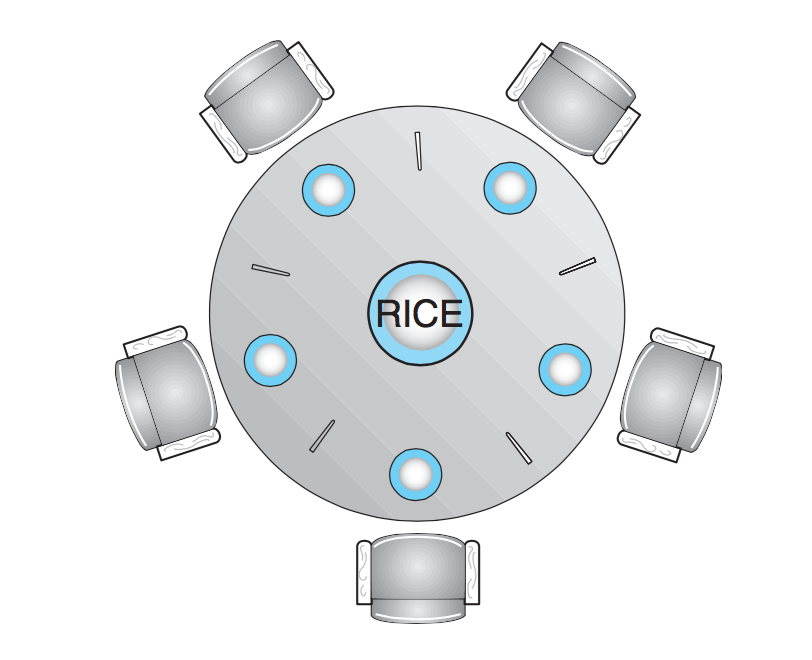
\includegraphics[width=0.4\textwidth]{images/philosopher-table.png}\\
The situation of the dining philosophers~\cite{osc}.
\end{center}

When a philosopher wishes to eat, she sits down at her designated chair, and attempts to pick up the two chopsticks that are nearest (one on the left, and one on the right). Philosophers are polite and therefore do not grab a chopstick out of the hands of a colleague. When a philosopher has both chopsticks, she may eat rice, and when she is finished, she puts down the chopsticks and goes back to thinking.

Humorous aside: as~\cite{mte241} points out, some textbooks formulate this problem as philosophers needing two forks to eat rather than chopsticks. It is, of course, much easier to imagine having difficulty eating with only one chopstick than having difficulty with only one fork. Of course, the scenario is a little bit silly. We don't study it because it is supposed to be a true to life model of how real philosophers behave. The scenario is just a convenient and memorable example of a whole class of problems.

Suppose then that semaphores are the method for managing things. Because only one person can be in possession of a chopstick at a time, each chopstick may be represented by a binary semaphore. As a philosopher needs the chopstick to his left and right to eat, when the philosopher sits down he attempts to acquire the left chopstick, then the right, eats, and puts the chopsticks down. This works fine, until all philosophers sit down at the same time. Each grabs the chopstick to his or her left. None of them are able to acquire the chopstick to his or her right (because someone has already picked it up). None of the philosophers can eat; they are all stuck. This is deadlock. 

This example makes it more clear why we call a situation where a thread never gets to run ``starvation''. If a philosopher is never able to get both chopsticks, that philosopher will never be able to eat, and though I am not an expert on biology, I have it on good authority that people who do not eat anything end up eventually starving to death. Even philosophers.

One thing that would guarantee that this problem does not occur is to protect the table with a binary semaphore. This would allow exactly one philosopher at a time to eat, but at the very least, deadlock and starvation would be avoided. Although this works, it is a suboptimal solution. There are five seats and five chopsticks and yet only one person is eating at a time. We can get better concurrency and use of the resources.

Next idea: what if we limit the number of philosophers at the table concurrently to four? The pigeonhole principle applies here: if there are $k$ pigeonholes and more than $k$ pigeons, at least one pigeonhole must have at least two pigeons. Thus, at least one of the four philosophers can get two chopsticks~\cite{mte241}. Implementing the solution is easy; we have a general semaphore with a maximum and initial value of 4.

Another idea: the problem above occurs because every philosopher tries to pick up the left chopstick first. If some of them try to pick up the left and some pick up the right first, then deadlock will not happen, either~\cite{osc}.

The dining philosophers problem is a good springboard from which to launch into a much deeper discussion of deadlock, and starvation; that is what we will examine next.

\bibliographystyle{alpha}
\bibliography{254}


\end{document}